\chapter{Zelené karty}
Zelené karty sa aktivujú až po skončení vášho ťahu. Ak si teda vyložíte napríklad kartu Sombrero, môžete ju použiť proti efektu Bang!, ktorý príde od ďalšieho hráča. Rovnako ako pri modrých kartách platí, že hráč nemôže mať vyložené dve zelené karty s rovnakým názvom.
\begin{comment}
\begin{figure}[!h]
\begin{minipage}[t]{\minipageSize}\centering
  \includegraphics[width=\cardSize\linewidth]{}
 \caption[]{}
  \label{fig:bang}
\end{minipage}
\hfill
\begin{minipage}[t]{\minipageSize}\centering
  \includegraphics[width=\cardSize\linewidth]{}
  \caption[]{}
  \label{fig:vedle}
\end{minipage}
\hfill
\begin{minipage}[t]{\minipageSize}\centering
  \includegraphics[width=\cardSize\linewidth]{}
  \caption[]{}
  \label{fig:duel}
\end{minipage}
\hfill
\begin{minipage}[t]{\minipageSize}\centering
  \includegraphics[width=\cardSize\linewidth]{}
\caption[]{}
  \label{fig:panico}
\end{minipage}
\end{figure}
\end{comment}

\begin{figure}[!h]
\begin{minipage}[t]{\minipageSize}\centering
  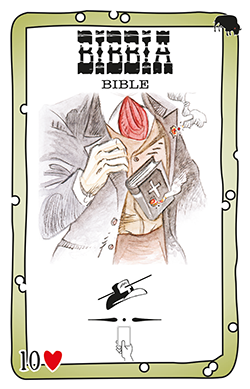
\includegraphics[width=\cardSize\linewidth]{Zelene/03_bibbia.png}
 \caption[Bible]{Vyvolá efekt Vedle!. Po použití si hráč potiahne 1 kartu.}
\end{minipage}
\hfill
\begin{minipage}[t]{\minipageSize}\centering
  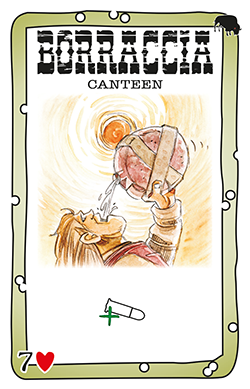
\includegraphics[width=\cardSize\linewidth]{Zelene/03_borraccia.png}
  \caption[Čutora]{Vyvolá efekt Pivo.}
  \label{fig:vedle}
\end{minipage}
\hfill
\begin{minipage}[t]{\minipageSize}\centering
  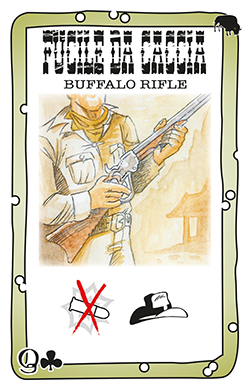
\includegraphics[width=\cardSize\linewidth]{Zelene/03_fucile_da_caccia.png}
  \caption[Puška na bizóny]{Vyvolá efekt Bang! na neobmedzený dosah.}
  \label{fig:duel}
\end{minipage}
\hfill
\begin{minipage}[t]{\minipageSize}\centering
  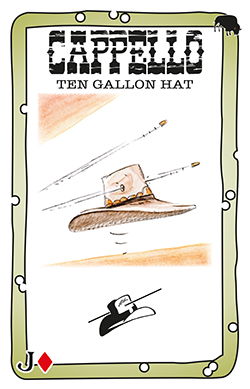
\includegraphics[width=\cardSize\linewidth]{Zelene/03_cappello.png}
\caption[Stetson]{Vyvolá efekt Vedle!.}
  \label{fig:panico}
\end{minipage}
\end{figure}

\begin{figure}[!h]
\begin{minipage}[t]{\minipageSize}\centering
  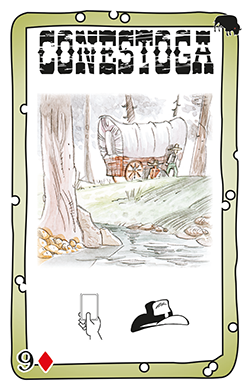
\includegraphics[width=\cardSize\linewidth]{Zelene/03_conestoga.png}
 \caption[Krytý vuz]{Hráč, ktorý túto kartu zahrá zoberie kartu ľubovoľnému hráčovi z ruky alebo z vyložených kariet na neobmedzený dosah. Dá sa zahrať iba vo svojom ťahu.}
  \label{fig:Vuz}
\end{minipage}
\hfill
\begin{minipage}[t]{\minipageSize}\centering
  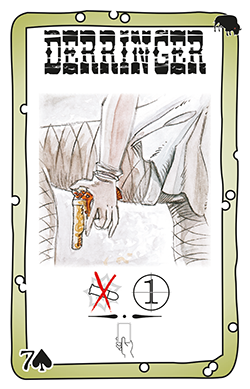
\includegraphics[width=\cardSize\linewidth]{Zelene/03_derringer.png}
  \caption[Derringer]{Vyvolá efekt Bang! na vzdialenosť 1 a hráč si potom potiahne 1 kartu bez ohľadu na výsledok. Vzdialenosť upravujú karty vyložené pred hráčmi.}
  \label{fig:vedle}
\end{minipage}
\hfill
\begin{minipage}[t]{\minipageSize}\centering
  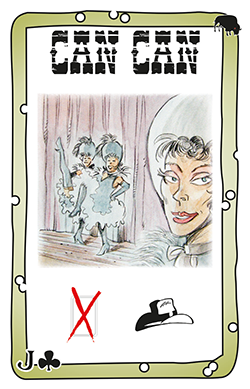
\includegraphics[width=\cardSize\linewidth]{Zelene/03_can_can.png}
  \caption[Kankán]{Hráč, ktorý zahrá túto kartu, odhodí ľubovoľnému hráčovi, na neobmedzený dosah kartu z ruky alebo kartu, ktorú ma vyloženú pred sebou. Je možné ju použiť len vo svojom ťahu.}
  \label{fig:duel}
\end{minipage}
\hfill
\begin{minipage}[t]{\minipageSize}\centering
  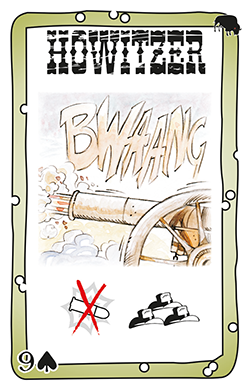
\includegraphics[width=\cardSize\linewidth]{Zelene/03_howitzer.png}
\caption[Houfnice]{Vyvolá efekt Bang! proti všetkým hráčom v hre. Nepočíta sa do limitu kariet Bang!.}
  \label{fig:panico}
\end{minipage}
\end{figure}

\begin{figure}[!h]
\begin{minipage}[t]{\minipageSize}\centering
  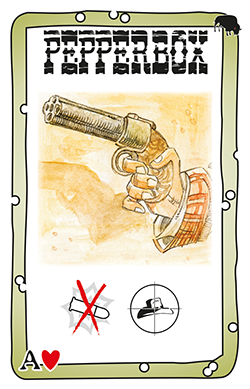
\includegraphics[width=\cardSize\linewidth]{Zelene/03_pepperbox.png}
 \caption[Pepperbox]{Vyvolá efekt Bang! na dostrel.}
  \label{fig:bang}
\end{minipage}
\hfill
\begin{minipage}[t]{\minipageSize}\centering
  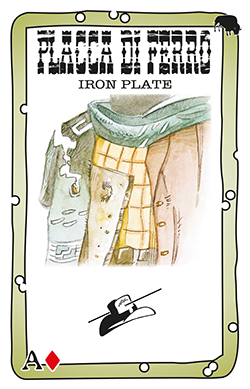
\includegraphics[width=\cardSize\linewidth]{Zelene/03_placca_di_ferro.png}
  \caption[Železný plát]{Vyvolá efekt Vedle!.}
  \label{fig:vedle}
\end{minipage}
\hfill
\begin{minipage}[t]{\minipageSize}\centering
  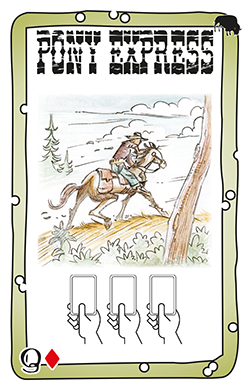
\includegraphics[width=\cardSize\linewidth]{Zelene/03_pony_express.png}
  \caption[Pony express]{Hráč si potiahne 3 karty.}
  \label{fig:duel}
\end{minipage}
\hfill
\begin{minipage}[t]{\minipageSize}\centering
  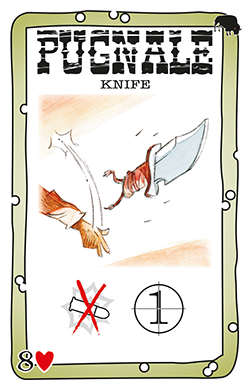
\includegraphics[width=\cardSize\linewidth]{Zelene/03_pugnale.png}
\caption[Nuž]{Vyvolá efekt Bang! na vzdialenosť 1. Vzdialenosť upravujú karty vyložené pred hráčmi.}
  \label{fig:panico}
\end{minipage}
\end{figure}

\begin{figure}[!h]
\begin{minipage}[t]{\minipageSize}\centering
  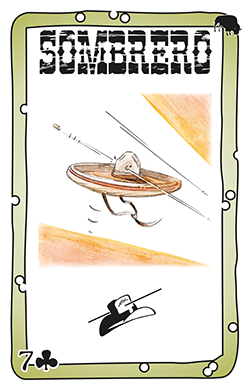
\includegraphics[width=\cardSize\linewidth]{Zelene/03_sombrero.png}
 \caption[Sombrero]{Vyvolá efekt Vedle!.}
  \label{fig:bang}
\end{minipage}
\hfill
\vfill
\end{figure}
